\section{Classification Trees and Random Forests}
% TODO: cleanup

\begin{sectionbox}
	\subsection{CART Algorithms}
	Generate Binary Trees by splitting $\mathbb X$ at each (internal/root) node: $\mathbb{X}_{i,left}=\{\vx\in\mathbb{X}_i|x_{j_i}<\tau_i\}\quad\mathbb{X}_{i,right}=\mathbb{X}_i\backslash\mathbb{X}_{i,left}$
	
	\textbf{Root/Internal node}: Binary decision based on chosen threshold $\tau_i\in\mathbb{R}$, feature $x_{j_i}=[\vx]_{j_i}$ with $j_i\in\mathbb{J}=\{1,...,dim[\mathbb{X}]\}$ aims at minimizing $Risk_{emp}(T_{CART})$
	
	\textbf{Terminal node}: $n_i$ corresponds to subset $\mathbb{X}_i\in\mathbb{X}$ $\rightarrow$ has no more children; outputs a decision
	
	$\Rightarrow \vx\mapsto n_i(\vx)$  
	
	\textbf{Example:}

	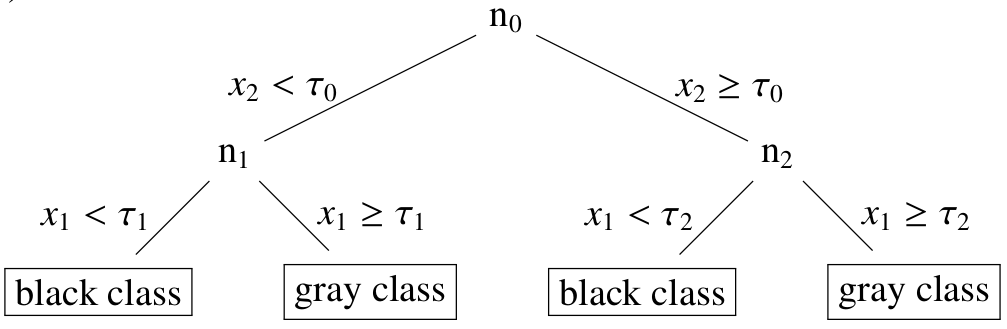
\includegraphics[width = 0.7\columnwidth]{CART_example}
	
\end{sectionbox}
\begin{sectionbox}
	
	\textbf{Empirical Impurity Measure}: choose $j_i$ and $\tau_i$ at $n_i$ by:
	$I_{CART}(\mathbb{S}_i)=\sum_{k=1}^{K}(1-\hat{P}_{Y|X}(Y=\theta_k|\{\vx\in\mathbb{X}_i\};\mathbb{S}_i))\hat{P}_{Y|X}(Y=\theta_k|\{\vx\in\mathbb{X}_i\};\mathbb{S}_i)$
	
	with\\ $\hat{P}_{Y|X}(Y=\theta_k|\{\vx\in\mathbb{X}_i\};\mathbb{S}_i)=\frac{M_k(\mathbb{S}_i)}{M(\mathbb{S}_i)}=\frac{|\{(\vx,y)\in\mathbb{S}_i|y=\theta_k\}|}{|\mathbb{S}_i|}$
	
	$\Rightarrow \{j_i,\tau_i\}=\underset{j\in\mathbb{J},\tau\in\mathbb{R}}{\operatorname{argmin}}\Big\{\sum_{k=1}^{K}\Big(1-\frac{M_k(\mathbb{S}_{i,left})}{M(\mathbb{S}_{i,left})}\Big)\frac{M_k(\mathbb{S}_{i,left})}{M(\mathbb{S}_{i})}+\Big(1-\frac{M_k(\mathbb{S}_{i,right})}{M(\mathbb{S}_{i,right})}\Big)\frac{M_k(\mathbb{S}_{i,right})}{M(\mathbb{S}_{i})}\Big\}$
	
	\textbf{Overfitting}(comes with high purity) can be controlled by a \textit{Test Set} $\mathbf{S}_{Test}$.\\
	\textbf{Decision Rule}: At terminal node $n_i$, input $\vx$ is assigned to $T_{CART}(\vx;\mathbb{S}):\mathbb{X}\mapsto \{1,...,K\}, \vx\mapsto \underset{k}{\argmax}\{M_k(\mathbb{S}_i)\}$\\
	
	\textbf{Gini Impurity Index}: $\boxed{I_{CART}}=\\\boxed{\sum_{k=1}^{K}(1-P_{Y|X}(\vec{y}=\theta_k|\{\vx\in\mathbb{X}\}))P_{Y|X}(\vec{y}=\theta_k|\{\vx\in\mathbb{X}\})}
	=\boxed{\sum_{k=1}^{K}\sum_{j=1,j\neq k}^{K}P_{Y|X}(\vec{y}=\theta_j|\{\vx\in\mathbb{X}\})P_{Y|X}(\vec{y}=\theta_k|\{\vx\in\mathbb{X}\})}$
	
	
\end{sectionbox}

\begin{sectionbox}
	\subsection{Random Forests}	
	Avoid \textit{Overfitting} (here: CART) $\Rightarrow$ combine independent \textit{Hypothesis Tests}: e.g. by \textit{Majority Vote}\\ $T_{maj}(\vx)=majority\{T_{CART}(\vx;\mathbb{S}^{(t)},\nu^{(t)})\}_{t=1}^{t_{max}}$\\
	\textit{Randomization Parameter} $\nu_t$ controls an additionally introduced
	Randomness between the individual Tests.\\
	$\Rightarrow$ \textit{Variance} of $T_{avg}(\vx)$ is reduced by 1/$t_{max}$ with respect to the \textit{Variance} of the individual test.
	
	\textbf{Random Forest Method}:
	\begin{itemize}
		\item $T_{RF}(\vx)=majority\{T_{CART}(\vx;\mathbb{S}^{(t)},\mathbb{J}^{(t)})\}_{t=1}^{t_{max}}$
		\item Stochastic Independence by Bootstrapping of training samples (random sampling from $\mathbb{S}$ with replacement) $\Rightarrow$ large $t_{max}$ guarantees excellent performance (yet Tests are still correlated)
		\item Overfitting not considered (maximum purity) $\Rightarrow$ small bias of RF Method
	\end{itemize}
\end{sectionbox}
